\documentclass[12pt,fleqn,answers]{exam}
\usepackage{pifont}
\usepackage{dingbat}
\usepackage{amsmath,amssymb}
\usepackage{epsfig}
\usepackage[super]{nth}
\usepackage[colorlinks=true,linkcolor=black,anchorcolor=black,citecolor=black,filecolor=black,menucolor=black,runcolor=black,urlcolor=black]{hyperref}
\usepackage[letterpaper, margin=0.5in]{geometry}
\addpoints
\boxedpoints
\pointsinmargin
\pointname{pts}
\usepackage{graphicx}
\usepackage[activate={true,nocompatibility},final,tracking=true,kerning=true,factor=1100,stretch=10,shrink=10]{microtype}
\usepackage[american]{babel}
%\usepackage[T1]{fontenc}
\usepackage{fourier}
\usepackage{isomath}
\usepackage{upgreek,amsmath}
\usepackage{amssymb}
\usepackage{graphicx}

\newcommand{\dotprod}{\, {\scriptzcriptztyle
    \stackrel{\bullet}{{}}}\,}

\newcommand{\reals}{\mathbf{R}}
\newcommand{\lub}{\mathrm{lub}} 
\newcommand{\glb}{\mathrm{glb}} 
\newcommand{\complex}{\mathbf{C}}
\newcommand{\dom}{\mbox{dom}}
\newcommand{\range}{\mbox{range}}
\newcommand{\cover}{{\mathcal C}}
\newcommand{\integers}{\mathbf{Z}}
\newcommand{\vi}{\, \mathbf{i}}
\newcommand{\vj}{\, \mathbf{j}}
\newcommand{\vk}{\, \mathbf{k}}
\newcommand{\bi}{\, \mathbf{i}}
\newcommand{\bj}{\, \mathbf{j}}
\newcommand{\bk}{\, \mathbf{k}}
\DeclareMathOperator{\Arg}{\mathrm{Arg}}
\DeclareMathOperator{\Ln}{\mathrm{Ln}}
\newcommand{\imag}{\, \mathrm{i}}

\usepackage{graphicx}
\usepackage{color}
\shadedsolutions
\definecolor{SolutionColor}{rgb}{0.8,0.9,1}
\newcommand\AM{\textsc{am}}
\newcommand\PM{\textsc{pm}}
     
\usepackage{utopia}

\newcommand{\quiz}{10}
\newcommand{\term}{Fall}
\newcommand{\due}{Wednesday 31 August at 13:15 \PM}
\newcommand{\class}{MATH 115}
\begin{document}



\vspace{0.1in}

\noindent \textbf{Week 10 FLO} (Friday Learning Opportunity) 

\begin{questions}  
    
 \question Given these facts about a function $J$, draw a sketch of $J$ that has all the given properties:
 
  \begin{tabular}{|c|c|}  \hline \hline 
 $ x < 2$  & $J^\prime(x) < 0$ \\  \hline
 $ 2 < x < 3$   & $J^\prime (x) = 0$ \\  \hline
  $ 3 < x $   & $J^\prime(x) > 0$  \\ \hline
 \end{tabular}
 
 Also $J(2) = 5$.
 
  \question Given these facts about a function $J$, draw a sketch of $J$ that has all the given properties:
  
  \begin{tabular}{|c|c|}  \hline  \hline
 $ x < 2$  & $J^\prime(x) > 0$ \\  \hline
   $ 2 < x $   & $J^\prime(x) < 0$\\  \hline
 \end{tabular}
 
 Also $J(2) = 5$ and $J$ is not differentiable at $2$.
 
 
 \question A graph of a function $V$ is shown.  As best you can, sketch a graph of $V^\prime$.
 
 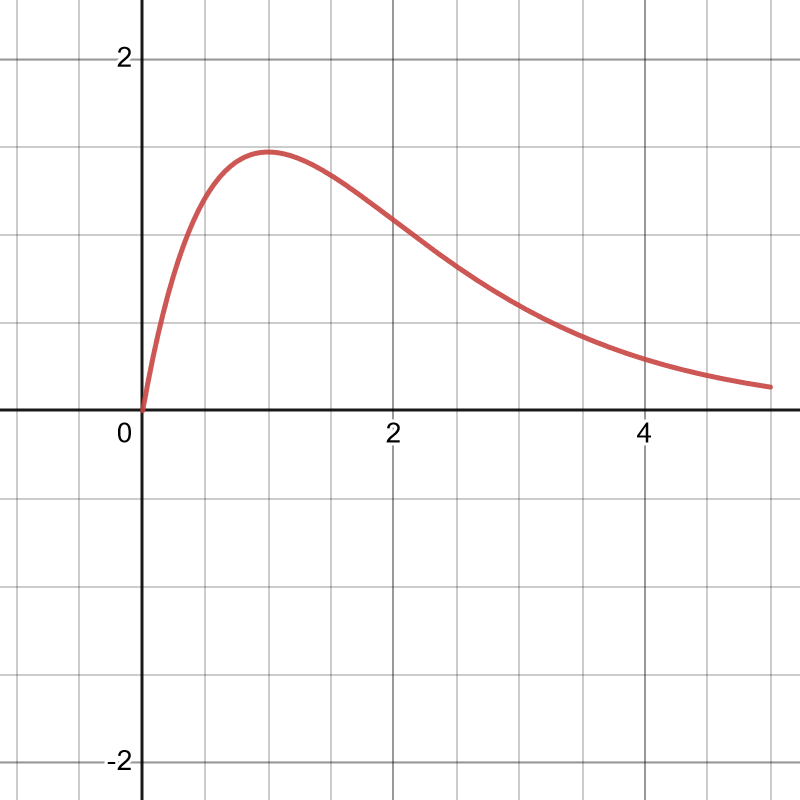
\includegraphics[scale=0.2]{desmos-graph(38)}
 
 \question For the function $T(x) = \frac{x+5}{x+7}$, solve the inequality  $T^\prime(x) > 0$; and solve the 
 inequality $T^{\prime \prime}(x) > 0$.
\end{questions}
\end{document}